%%%%%%%%%%%%%%%%%
% This is an sample CV template created using altacv.cls
% (v1.3, 10 May 2020) written by LianTze Lim (liantze@gmail.com). Now compiles with pdfLaTeX, XeLaTeX and LuaLaTeX.
%
%% It may be distributed and/or modified under the
%% conditions of the LaTeX Project Public License, either version 1.3
%% of this license or (at your option) any later version.
%% The latest version of this license is in
%%    http://www.latex-project.org/lppl.txt
%% and version 1.3 or later is part of all distributions of LaTeX
%% version 2003/12/01 or later.
%%%%%%%%%%%%%%%%

%% If you are using \orcid or academicons
%% icons, make sure you have the academicons
%% option here, and compile with XeLaTeX
%% or LuaLaTeX.
% \documentclass[10pt,a4paper,academicons]{altacv}

%% Use the "normalphoto" option if you want a normal photo instead of cropped to a circle
% \documentclass[10pt,a4paper,normalphoto]{altacv}

\documentclass[10pt,a4paper,ragged2e,withhyper]{altacv}

%% AltaCV uses the fontawesome5 and academicons fonts
%% and packages.
%% See http://texdoc.net/pkg/fontawesome5 and http://texdoc.net/pkg/academicons for full list of symbols. You MUST compile with XeLaTeX or LuaLaTeX if you want to use academicons.

% Change the page layout if you need to
\geometry{left=1.1cm,right=1cm,top=1.5cm,bottom=1.5cm,columnsep=1.2cm}

% The paracol package lets you typeset columns of text in parallel
\usepackage{paracol}

% Change the font if you want to, depending on whether
% you're using pdflatex or xelatex/lualatex
\ifxetexorluatex
  % If using xelatex or lualatex:
  \setmainfont{Roboto Slab}
  \setsansfont{Lato}
  \renewcommand{\familydefault}{\sfdefault}
\else
  % If using pdflatex:
  \usepackage[rm]{roboto}
  \usepackage[defaultsans]{lato}
  \usepackage{graphicx}
  % \usepackage{sourcesanspro}
  \renewcommand{\familydefault}{\sfdefault}
\fi

% Change the colours if you want to
\definecolor{VividPurple}{HTML}{3E0097}
\definecolor{SlateGrey}{HTML}{2E2E2E}
\definecolor{LightGrey}{HTML}{666666}
\colorlet{name}{black}
\colorlet{tagline}{VividPurple}
\colorlet{heading}{VividPurple}
\colorlet{headingrule}{VividPurple}
\colorlet{subheading}{VividPurple}
\colorlet{accent}{VividPurple}
\colorlet{emphasis}{SlateGrey}
\colorlet{body}{LightGrey}

% Change some fonts, if necessary
\renewcommand{\namefont}{\Huge\rmfamily\bfseries}
\renewcommand{\personalinfofont}{\footnotesize}
\renewcommand{\cvsectionfont}{\LARGE\rmfamily\bfseries}
\renewcommand{\cvsubsectionfont}{\large\bfseries}


% Change the bullets for itemize and rating marker
% for \cvskill if you want to
\renewcommand{\itemmarker}{{\small\textbullet}}
\renewcommand{\ratingmarker}{\faCircle}

%% sample.bib contains your publications
% \addbibresource{sample.bib}

\begin{document}
\name{Edouard Legoupil}
\tagline{Information Management, AI \& Data Science for Evidence Building}
%% You can add multiple photos on the left or right
\photoR{2.8cm}{edouard_pic.jpg}
% \photoL{2.5cm}{Yacht_High,Suitcase_High}

\personalinfo{%
  % Not all of these are required!
  \email{edouard.legoupil@gmail.com}
  \phone{+34-645-025115}
 % \mailaddress{Åddrésş, Street, 00000 Cóuntry}
  \location{Valencia, Spain}
 % \homepage{www.homepage.com}
  \twitter{edouard\_lgp}
  \linkedin{edouardlegoupil}
  % \github{edouard-legoupil}
  %% You MUST add the academicons option to \documentclass, then compile with LuaLaTeX or XeLaTeX, if you want to use \orcid or other academicons commands.
  % \orcid{0000-0000-0000-0000}
  %% You can add your own arbtrary detail with
  %% \printinfo{symbol}{detail}[optional hyperlink prefix]
  % \printinfo{\faPaw}{Hey ho!}[https://example.com/]
  %% Or you can declare your own field with
  %% \NewInfoFiled{fieldname}{symbol}[optional hyperlink prefix] and use it:
  % \NewInfoField{gitlab}{\faGitlab}[https://gitlab.com/]
  % \gitlab{your_id}
}

\makecvheader
%% Depending on your tastes, you may want to make fonts of itemize environments slightly smaller
% \AtBeginEnvironment{itemize}{\small}

%% Set the left/right column width ratio to 6:4.
\columnratio{0.6}

% Start a 2-column paracol. Both the left and right columns will automatically
% break across pages if things get too long.
\begin{paracol}{2}
\cvsection{Experience}

\cvevent{Chief Data Officer, ICT Division}{IOM, International Organisation for Migration - P5}{Jul 2024 -- Ongoing}{Valencia, Spain}
\begin{itemize}
\item Supported the roll-out of a data literacy program focusing on data story telling.
\item Implemented a data mesh architecture for cross-domain analytics.  
\item Supported the establishment of data governance monitoring tools.  
\item Developed an AI multi-agent system to handle internal processes.

\end{itemize}

\divider

\cvevent{Senior Regional Evaluation Officer, Regional Bureau for the Americas}{UNHCR, United Nations High Commissioner for Refugees - P4}{Jan 2024 -- June 2024}{Ciudad del Saber, Panama}
\begin{itemize}
\item Scope and Manage Country Strategy Evaluation Studies
\item Prototype an AI System to re-inject Evidence Learning within multiyear Strategic Plan using Retrieval Augmented Generation (RAG).

\end{itemize}

\divider

\cvevent{Senior Regional Data Analysis Officer, Regional Bureau for the Americas}{UNHCR, United Nations High Commissioner for Refugees - P4}{Jan 2020 -- Dec 2023}{Ciudad del Saber, Panama}
\begin{itemize}
\item Deploy harmonized high frequency household survey program.  
\item Support calibration of composite indicators for vulnerability.

\end{itemize}

\divider

\cvevent{Senior Information Management Officer, Emergency Deployment for Hurricane Dorian}{Global Protection Cluster, United Nations - P4}{Sept 2019 -- Dec 2019}{Nassau \& Marsh Harbour, The Bahamas}
\begin{itemize}
\item Advised Government and responding organizations on Emergency Registration System \& Procedures for Affected Population.  
\item Contributed to Humanitarian Severity Assessment \& Analysis.

\end{itemize}

\divider

\cvevent{Senior Regional Information Management Officer, Regional Bureau for Middle East \& North Africa}{UNHCR, United Nations High Commissioner for Refugees - P4}{June 2015 -- August 2019}{Amman, Jordan}
\begin{itemize}
\item Regional support on Needs Assessment, Targeting \& Situation Analysis.  
\item Statistical analysis of sample based household surveys.

\end{itemize}

\divider

\cvevent{Information Management Officer, Jordan Operation}{UNHCR, United Nations High Commissioner for Refugees - P3}{June 2013 -- May 2015}{Amman, Jordan}
\begin{itemize}
\item Situation and response analysis for an Emergency influx 600,000 Syrian refugees.
\item Set-up of a coordinated system with more than 60 Non-Government Organizations to collect, track \& visualize humanitarian activities for annual Refugee Response Plan.
\end{itemize}
\divider
\cvevent{Data Management Officer, Global Service Center}{UNHCR, United Nations High Commissioner for Refugees - P2}{Jan 2009 --  May 2013}{Budapest, Hungary}
\divider
\cvevent{Regional GIS Officer, Regional Expert Hub for Western Africa}{UNHCR, United Nations High Commissioner for Refugees - JPO}{Nov 2005 -- Dec 2008}{Accra, Ghana}
\divider
\cvevent{Project Manager: GIS \& Land Management}{Local Government of French Guyana, Regional Nature Park}{Jun 2004 -- Sept 2005}{Cayenne, French Guyana} 
\divider
\cvevent{Food Aid Manager (8,000 metric tons of wheat)}{Burundian Ministry of Agriculture \& French Embassy in Burundi }{Jun 2000 -- Dec 2001}{Bujumbura, Burundi}

\divider 

\cvevent{Researcher on Agricultural Market \& Food Industry }{MADERA - Non Governmental Organization}{Jun 1999 -- Nov 1999}{Jalalabad, Afghanistan}



\medskip

% \cvsection{A typical working day}

% Adapted from @Jake's answer from http://tex.stackexchange.com/a/82729/226
% \wheelchart{outer radius}{inner radius}{
% comma-separated list of value/text width/color/detail}
% \wheelchart{1.5cm}{0.5cm}{%
%   13/10em/accent!20/\footnotesize Sleep,
%   3/13em/accent!10/\footnotesize\\[1ex] Sport,
%   22/9em/accent!60/Research \& Resolve issues with Operations,
%   15/9em/accent!40/\footnotesize Coach \& Support technical colleagues,
%   28/9em/accent/ Participate in brainstorming meetings,
%   14/7em/accent!20/\footnotesize\\[1ex]Spend time with my wife \& 3 daughters,
%   5/3em/accent!40/\footnotesize\\[1ex] Coding data tools
% }

% use ONLY \newpage if you want to force a page break for
% ONLY the current column


%% Switch to the right column. This will now automatically move to the second
%% page if the content is too long.
\switchcolumn

\cvsection{Slogan}
\begin{quote}
``Without data, you’re just another person with an opinion'' \footnotesize W. Edwards Deming 
\end{quote}
\divider
\begin{quote}
``Without an opinion, you’re just another person with data'' \footnotesize Peter Drucker. 
\end{quote}


\cvsection{Credited for}

\cvachievement{\faSlideshare}{Enhancing Data Literacy}{Built a \href{https://unhcr.github.io/koboloadeR/docs/}{knowledge base}, a \href{https://unhcr.github.io/koboloadeR/docs/}{package} and a \href{https://humanitarian-user-group.github.io/post/first-meeting/}{user community} to enhance capacity to make the most of available data to support humanitarian operations.}

\divider 

\cvachievement{\faBullseye }{Protection Vulnerability Scoring}{Designed an innovative conceptual approach \& measurement model to target \& articulate humanitarian assistance.}

\divider

\cvachievement{\faTrophy}{Received UNHCR Innovation Award}{For performed technical leadership on the development and launch of  \href{http://data.unhcr.org}{Operational Data Portal} Platform}


\cvsection{Strengths}


\cvtag{Solution-oriented}
\cvtag{Cultural-sensitive}
\cvtag{Creative-thinking}
\cvtag{Project-management}

\cvsection{ Languages}

\cvskill{English- C2}{6}
\cvskill{French - C2}{6}
\cvskill{Spanish - B2}{4}
\cvskill{German - A2}{2}
\cvskill{Arabic - A1}{1}
\cvskill{R-STAT Language}{6}
\cvskill{Python - LLM/RAG}{4}

%% Yeah I didn't spend too much time making all the
%% spacing consistent... sorry. Use \smallskip, \medskip,
%% \bigskip, \vpsace etc to make ajustments.
\medskip

\cvsection{Digital Skills}

\cvevent{Evidence-based Decision Support}{Data Collection Design, Data Mining, Data Visualisation, Collaborative Data Interpretation and Business Intelligence}{}{} 

\cvevent{Persuasive Communication}{Presenting complex topics to broad \& diverse audience in simple terms using didactic materials and effective visuals}{}{}

\cvevent{Social Media \& Web}{Syndicating technical knowledge and academic literature review for professional experts}{}{}
 


\cvsection{Education}

\cvevent{M.S.\ in Geographic Information System Architecture \& Cartography}{ENSG, France}{Sept 2003 -- June 2004}{}

\divider

\cvevent{M.S.\ in International Agro-Economics \& Rural Development}{ISTOM, France}{Sept 1998 -- June 2001}{}

\divider

\cvevent{B.S.\ in Economics, Business Administration, Finance, Accounting}{Université de Nantes, France}{Sept 1996 -- June 1998}{}

\divider

\cvevent{Classes Prépa.\ - Hypokhâgne BL : Philosophy, Sociology \& Economics}{Lycée Guist'hau , France}{Sept 1995 -- June 1996}{}

% \divider




\end{paracol}

\cvsection{Exposure to Cultural Diversity }

Both for work and personal interest

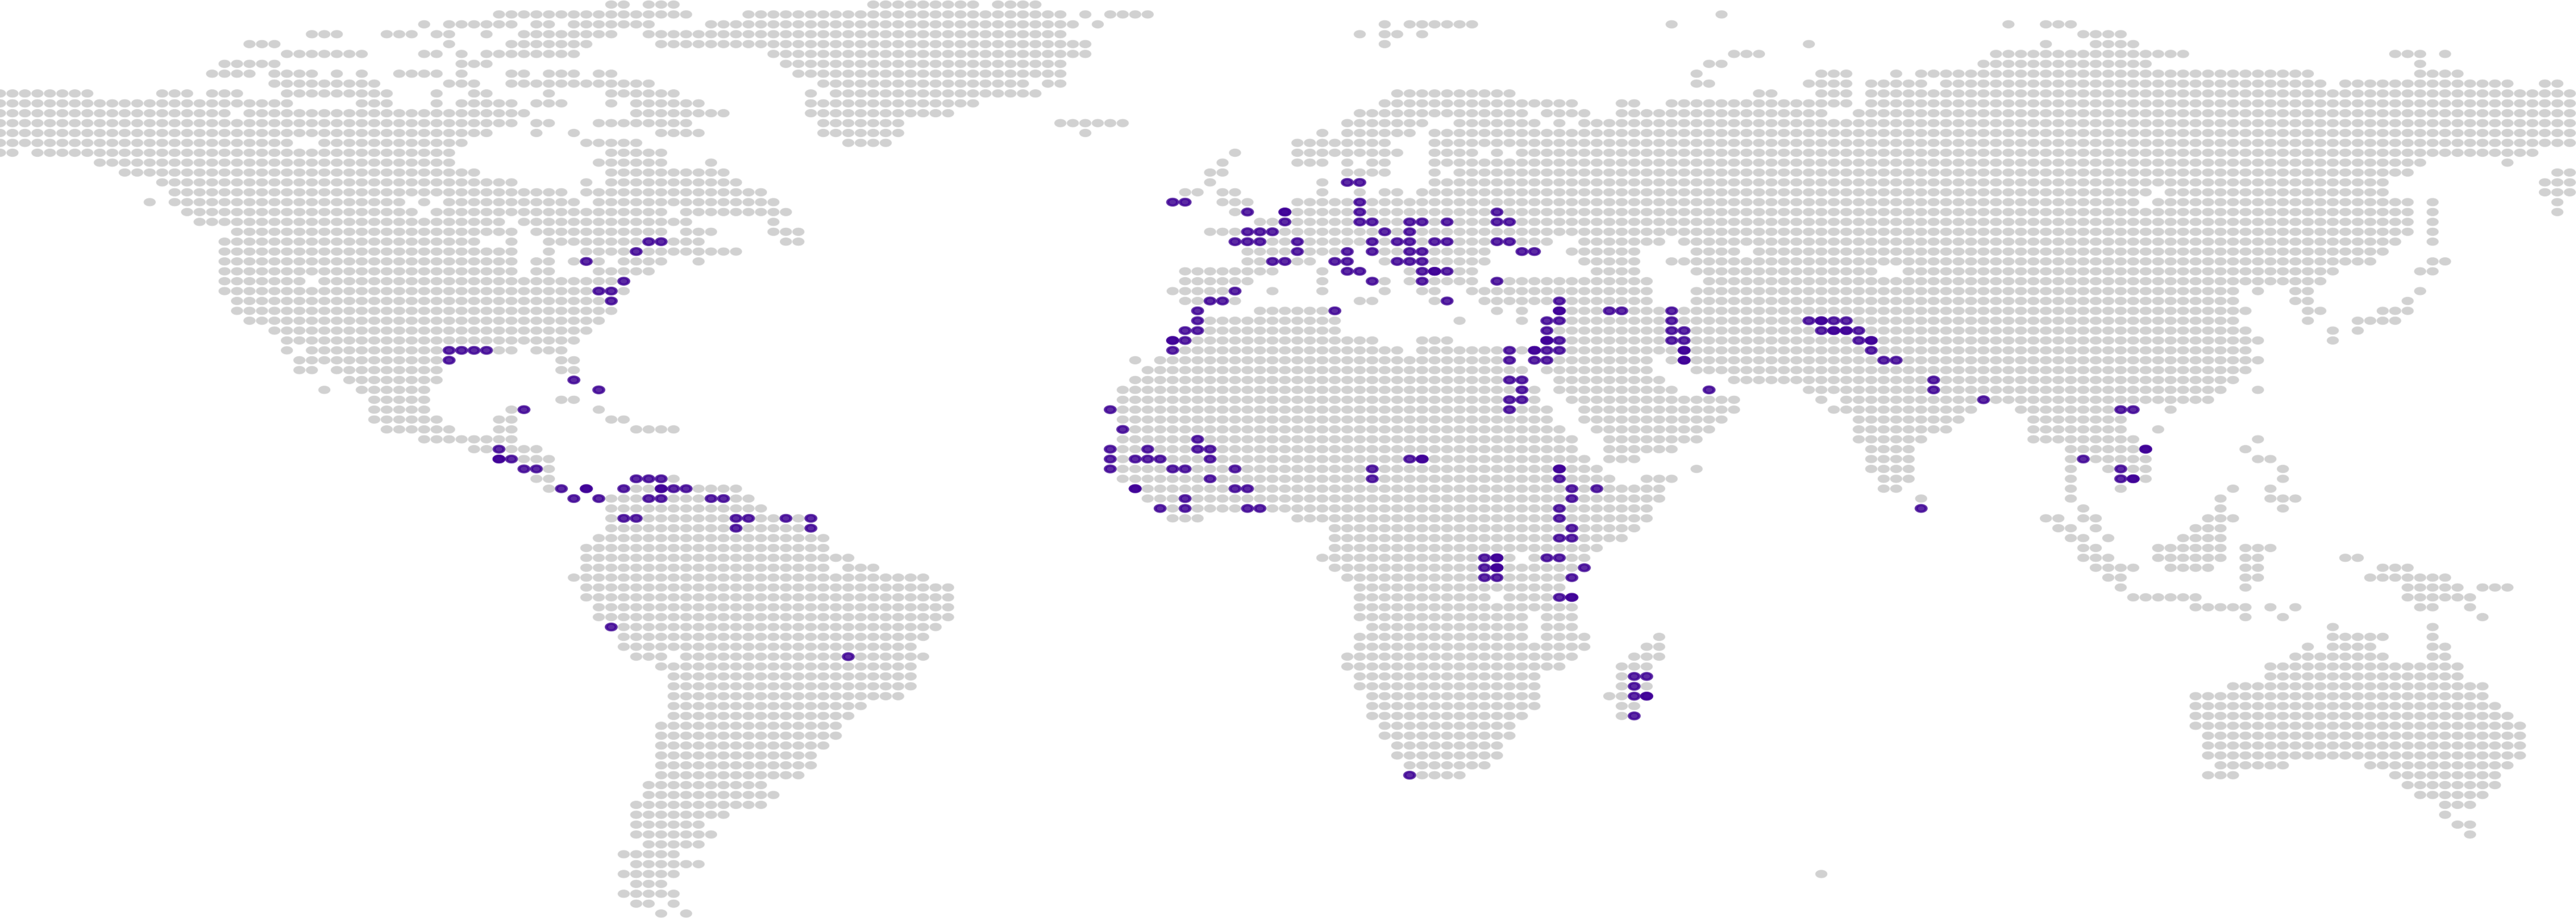
\includegraphics[width=\textwidth]{visited2024_1.png}


%% # https://taraskaduk.com/posts/2017-11-26-pixel-maps/
%% ### setup ----------------------------------------------------------------------
%% # install and/or load packages
%% pkg <- c("tidyverse", "maps", "geonames", "sp", "sf","nngeo"  )
%% sapply(pkg, function(x){
%%   if(! x %in% installed.packages()) install.packages(x)
%%   require(x, character.only = TRUE)})
%% rm(pkg)

%% ### dot world grid -------------------------------------------------------------------
%% # generate worldwide dots
%% dots <- tibble(lat = seq(-89.5, 89.5, by = 1.5)) |>
%%   merge(tibble(long = seq(-180, 180, by = 1.5)), all = TRUE) |> 
%%   # exclude water-based dots 
%%   mutate(country = map.where('world', long, lat),
%%          lakes = map.where('lakes', long, lat)) |>
%%   filter(!is.na(country) 
%%          & is.na(lakes)  
%%          & lat > -65    
%%         & lat < 85   
%%          & lat > -150   
%%          & lat > -150 
%%          & country != "Antarctica") |>
%%   select(-lakes)
%% dot_sp <- sp::SpatialPointsDataFrame( coords = dots[ ,c("long","lat")] , data = dots)
%% dot_sf <- st_as_sf(dot_sp)
%% plot(dot_sf$geometry)

%% ### Location to geocode to grid -------------------------------------------------------------------
%% # https://docs.google.com/spreadsheets/d/1iyWkr7kGhHCNNBq3aaph782bHM2MHguVZeZMWqVQe24/edit#gid=0
%% locations <- read.csv("locations2023.csv")
%% locations_sp <- sp::SpatialPointsDataFrame( coords = locations[ ,c("lng","lat")] , 
%%                                             data = locations)
%% locations_sf <- st_as_sf(locations_sp)
%%  # Find nearest polygon per point
%% dot_location <- sf::st_join(dot_sf, 
%%                        locations_sf, 
%%                        join = nngeo::st_nn, 
%%                        maxdist = 1.2, 
%%                        k = 4, 
%%                        progress = FALSE) |> 
%%        dplyr::filter( !(is.na(flag)))

%% dot_map2 <-  ggplot() +   
%%   #base layer of map dots
%%   geom_point(data = dots, 
%%              aes(x=long, y = lat), 
%%              col = "#d1d1d1",
%%              size = 0.6)  + 
%%   # put france
%%   geom_point(data = dots |> filter( country == 'France'), 
%%              aes(x=long, y = lat),  
%%              color="#3E0097", 
%%              alpha = 0.8,
%%              size=0.7) +
%%   # put Jordan
%%   geom_point(data = dots |> filter( country == 'Jordan'), 
%%              aes(x=long, y = lat),  
%%              color="#3E0097", 
%%              alpha = 0.8,
%%              size=0.7) +
%%   # put Panama
%%   geom_point(data = dots |> filter( country == 'Panama'), 
%%              aes(x=long, y = lat),  
%%              color="#3E0097", 
%%              alpha = 0.8,
%%              size=0.7) +
%%   #plot all the places I've been to
%%   geom_point(data = dot_location , 
%%              aes(x=long, y=lat.x), 
%%              color="#3E0097", 
%%              alpha = 0.8,
%%              size=0.7) +
%%   #plot all the places I've been to
%%   # geom_point(data = locations_sf ,
%%   #            aes(x=lng, y=lat),
%%   #            color="#FFBF00",
%%   #            alpha = 0.5,
%%   #            size=0.9) +
%%   scale_y_continuous(limits = c(-65, 85), expand = c(0,0)) +
%%   scale_x_continuous(limits = c(-150,160), expand = c(0,0))   + 
%%   theme_void() +
%%   theme(panel.border = element_blank(),
%%         panel.background = element_blank(),
%%         plot.margin = unit(c(0, 0, 0, 0), "cm"))
%% dot_map2

%% ### Save to file-------------------------------------------------------------------
%% ggsave(here::here("visited2023.png"), 
%%        dot_map2, 
%%        dpi = 600, 
%%        width = 8, 
%%        height = 4.5)

\end{document}